\documentclass[a4paper,12pt]{article}
\usepackage[utf8]{inputenc}
\usepackage{graphicx}
\usepackage{multicolumn}
\usepackage{multirow}
\usepackage{booktabs}
\usepackage[indent=0pt,skip=3mm]{parskip}
\usepackage{array}
\usepackage{commath} % for abs ||
\usepackage{listings}             % Include the listings-package
\usepackage{tabs}
\usepackage{mathtools}
% \usepackage{colortbl}
% \usepackage{url}
\usepackage{hyperref}
\usepackage{datetime}
\usepackage[ top=5cm, left=1.5cm, right=1.5cm, headheight=4cm,bottom=0.5cm]{geometry}
\usepackage{lastpage} % include last page numbering
\usepackage{fancyhdr}
\usepackage[table]{xcolor}% ctan.org/pkg/xcolor %FOR COLORS
% \usepackage{frame}
\settimeformat{xxivtime}
\setdefaultdate{\ddmmyyyydate}
\hyphenation{matriz}
\graphicspath{{figures/}{./images/}}
\newcommand{\eq}[1]{$#1$}
\newcommand{\head}[1]{{\bfseries #1}}
\newcommand{\header}[2][\tiny]{{\bfseries #1 #2}}

%%%%%%%%%%%%%%%%%%%%%%%%%%%%%%%%%%%%%%%%%%%%%%%%%%%%%%%%%%%%%%%%%%%%%%
%%%%%%%%%%%%%%%%%%%%%%%%%%%%%%%%%%%%%%%%%
\newsavebox{\mytabularheader}
\newsavebox{\mytabularheadertitle}
\setlength{\extrarowheight}{0.1cm}
%----------------------------------------------------------------------------------
%-----------------------------------------------------------------------------------------------
\sbox{\mytabularheadertitle}{%
  \begin{minipage}{.52\textwidth}
    \begin{center}
        \bfseries \scriptsize  UNIVERSIDAD NACIONAL DE SAN AGUSTIN\\
        FACULTAD DE INGENIERÍA DE PRODUCCIÓN Y SERVICIOS\\
        ESCUELA PROFESIONAL DE INGENIERÍA DE SISTEMA\\[3mm]
    \end{center}
  \end{minipage}
}

\sbox{\mytabularheader}{%
    \begin{minipage}{\textwidth}
        \centering
        \begin{tabular}{cp{8cm}c}
            
\includegraphics[scale=0.3]{epis_logo.png} & 
            \usebox{\mytabularheadertitle} &
            
\includegraphics[scale=0.04]{abet_logo.png} \\
            % \hline
             &\multicolumn{1}{c}{Aprobación:  2022/03/01 Código: GUIA-PRLE-001} &  \\
        \end{tabular}
    \end{minipage}
}
%---------------------------------------
\renewcommand{\headrulewidth}{0pt}
\fancypagestyle{plain}{%
  \fancyhf{}%
  \fancyhf[ch]{\usebox{\mytabularheader}}
}
%--------------------------------------
\pagestyle{plain}
\definecolor{blackRed}{cmyk}{0,81,76,31}
%%%%%%%%%%%%%%%%%%%%%%%%%%%%%%%%%%%%%%%%%%%%%%%%%%%%%%%%%%%%%%%%%%%%%%%%%%%%%%%%%%%%%%%%%%

\begin{document}    
\lstset{language=Python,frame=single, firstnumber=1,basicstyle=\footnotesize,
numbers=left,showspaces=false,showstringspaces=false}   
    \title{Autómatas celulares\\Física Computacional}
    \date{\vspace{-5ex}}
    \maketitle
    \begin{center}
        Escrito por:\\
        Alván Ventura, Edsel Yael\\ \texttt{ealvan@unsa.edu.pe}
        \\[3mm]
        Docente:\\Apaza Veliz, Danny Giancarlo\\ \texttt{dapazav@unsa.edu.pe}\\[3mm]
        \today
    \end{center}
    % \newgeometry{top=2cm}
    \enlargethispage{\baselineskip}

\section{Introducción}
Los automatas celulares nacieron con Von Neuman\cite{cita1} en 1903, al
intentar modelar una máquina capaz de autoreplicarse. 
En este sentido, Von Neuman también buscó reglas para 
lograr este fin. 

Posteriormente Stanishlaw Ulam\cite{cita1} consideró
un arreglo de celdas en las cuales se podía tener
uno de los finitos estados permitidos y conforme pasaba el tiempo
las celdas tenian la posibilidad de cambiar de acuerdo a
funciones de transición. Luego en 1966 se publicó ``Theory of Self-Reproducing Automata''
por el estudiante de doctorado W. Burks.

En este sentido, se creó el término Autómata Celular, el cual se puede definir como\cite{cita2}:
\begin{quotation}
    \centering
    \emph{Un modelo matemático para un sistema dinámico compuesto por un conjunto de celdas o células que adquieren distintos estados o valores}
\end{quotation}
Se considera por tanto a un Automáta Celular(AC), como un sistema complejo discretizado
con respecto a sus estados finitos y a cada unidad de tiempo transcurrido. 
Además tiene la dificultad de no saber con exactitud
cual es la tendencia y propiedades de un AC dado un estado inicial. 
Pues a cada unidad de tiempo todas las celdas pueden cambiar de estado.

\section{Automáta Celular}
El automáta celular tiene un comportamiento basado en las configuraciones iniciales
y las reglas que dominan el cambio de sus estados finitos, resultando importante saber qué
elementos intervienen en un Autómata Celular, es por esto, que se hablará
de los componentes principales de los AC.
\newpage
\subsection{Elementos de un AC}
Un Automata Celular esta denotado por\cite{cita1}:
\begin{equation}
  AC(L, S, N, f)
\end{equation}
Donde:
\begin{table}[h]
    \centering
    \begin{tabular}{cp{10cm}}
        \toprule
        \head{Elementos} & \head{Descripción}\\
        \midrule
        \emph{L} & Es el espacio con una dimension ``n'', donde se desarrolla el AC. Considerando que cada elemento es una célula.\\
        \emph{S} & Es el conjunto finito de estados permitidos en AC, y cada célula debe adoptar uno de estos valores.\\
        \emph{N} & Es el conjunto de celulas que se consideran vecinas de una célula.
        Cuando el espacio es uniforme, la vecindad de cada célula tiene el mismo aspecto(isomorfismo).\\
        \emph{f} & Es la función de transición entre un estado a otro. Define principalmente como
        un estado siguiente es influenciado por su vecindad y su estado anterior.  \eq{f: S^N -> S}\\
        \bottomrule            
    \end{tabular}
\end{table}

\subsection{Tipos de límites de espacio.}
Existen 3 tipos de espacio segun Fernández\cite{cita2}:
    \begin{enumerate}
        \item \head{Fronteras periódicas:} Cuando una célula llega al límite del espacio, la célula que está
        al opuesto extremo del espacio es considerada su vecina, tanto para verticalmente como horizontalmente.
        Por lo tanto, la figura de un plano con estas condiciones se llama \emph{toroide}. 
        \item \head{Fronteras absorventes:} También llamadas fronteras abiertas\cite{cita2}, son las que consideran que el espacio es
        finito, y por lo tanto, las células en el límite del espacio no tienen vecindades en esa dirección.
        \item \head{Fronteras reflectantes:} En este tipo de frontera, las células en el limite del espacio toman
        valores dentro del espacio, como si se tratase de un espejo, pues replican los valores que están dentro del espacio.    
    \end{enumerate}
\begin{figure}[h]
    \centering
    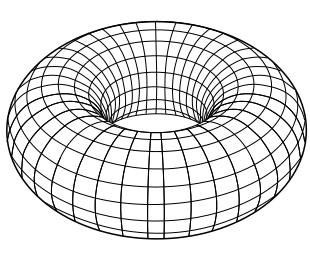
\includegraphics[width=0.3\textwidth]{torus.png}
    \caption{Reprensentación de una frontera periódica.}
\end{figure}

\newpage
\section{El juego de la vida.}

El juego de la vida esta implementado en un Automata Celular, que dadas sus condiciones
iniciales podemos observar como evoluciona el sistema en conjunto.

Al igual que un AC, podemos decir que tiene los siguientes componentes:

\begin{table}[h]
    \centering
    \begin{tabular}{cp{9cm}}
        \toprule
        \head{Elementos} & \head{Descripción}\\
        \midrule
        \emph{L} & El espacio esta determinado por NxN, donde \eq{N} es el número de celulas en 
        su dimension, que puede ser de una dimension \eq{d} determinada.\\
        \emph{S} & El conjunto finitos de estados son:
        \begin{itemize}
        \item \head{ON:} La célula esta viva.
        \item \head{OFF:} La célula esta muerta.
        \end{itemize}\\
        \emph{N} & Se considera que cada célula tendra en total 8 vecinos adyacentes tanto vertical como horizontalmente.\\
        \emph{f} & Y que la función de transición tendrá las siguientes 4 reglas:
        \begin{enumerate}
          \item \head{Primera regla:} Cualquier celda viva con menos de dos vecinas vivas muere.
          \item \head{Segunda regla:} Cualquier celda viva con dos o tres vecinos vivos vive.
          \item \head{Tercera regla:} Cualquier celda viva con más de tres vecinos vivos muere.
          \item \head{Cuarta regla: }Cualquier celda muerta con exactamente tres vecinos vivos se convierte en una celda viva.
        \end{enumerate}\\
        \bottomrule            
    \end{tabular}
\end{table}

\subsection{Implementación en Python}
El proceso principal del juego de la vida es\cite{cita3}:
\begin{enumerate}
    \item Inicializar las celdas en la cuadrícula.
    \item A cada paso del tiempo, para cada celda \eq{(i, j)}:
    \begin{enumerate}
        \item Actualice el valor de la celda \eq{(i, j)} en función de sus vecinos, 
        teniendo en cuenta las condiciones de contorno.
        \item Actualice los valores de la cuadrícula en cada paso del tiempo.
    \end{enumerate}
\end{enumerate}
\clearpage
El siguiente código es sacado por un repositorio de Github\footnote{https://github.com/electronut/pp/blob/master/conway/conway.py}
creado por Mahesh Venkitachalam.

\lstinputlisting[title=The Game of Life]{vida_game.py}

\subsubsection{Análisis}

El juego de la vida del script presentado en la anterior sección esta hecho
con las siguientes herramientas:
\begin{itemize}
    \item La librería \emph{numpy}, para los arreglos y cuadriculas del espacio de \emph{NxN}
    \item La librería \emph{matplotlib}, para el dibujo y la representación de la cuadricula.
    \item La librería \emph{argparse} para aceptar parametros via comandos.
\end{itemize}
\clearpage
Para empezar en el script anterior se presentan 3 tipos de condiciones iniciales las cuales son:
\begin{enumerate}
    \item La \emph{Glider}\cite{cita4}, es un patrón que es la primera nave espacial más pequeña, más común y descubierta por primera vez en el Juego de la Vida.
    \item La \emph{Gosper Glider Gun}\cite{cita5}, que configura el primer patrón finito conocido con crecimiento ilimitado, encontrado por Bill Gosper en noviembre de 1970.
    \item Y finalmente, el aleatorio, en el que se configura que una celda esta viva o muerta aleatoriamente.
\end{enumerate}
En la siguiente pieza de código se especifica que tipo de configuración inicial se decide, 
de acuerdo al parametro \emph{--glider}, \emph{--gosper} y si no se proporciona ninguna de esta se elige la opcion aleatoria.
\begin{lstlisting}
# viendo cual condicion inicial se elige
if args.glider:
    #primera opcion->glider
    grid = np.zeros(N*N).reshape(N, N)
    addGlider(1, 1, grid)
elif args.gosper:
    #segunda opcion -> gosper Gun
    grid = np.zeros(N*N).reshape(N, N)
    addGosperGliderGun(10, 10, grid)
else: 
    #tercera opcion-> aleatorioamente
        #mas vivos que muertos
    grid = randomGrid(N)
\end{lstlisting}

Para la \eq{1^{ra}} opción resulta con el comando:
\begin{quotation}
    \centering
    {\bfseries \ttfamily python vida\_game.py --grid-size 32 --interval 500 --glide}
\end{quotation}

El resultado es:
\begin{figure}[h]
    \centering
    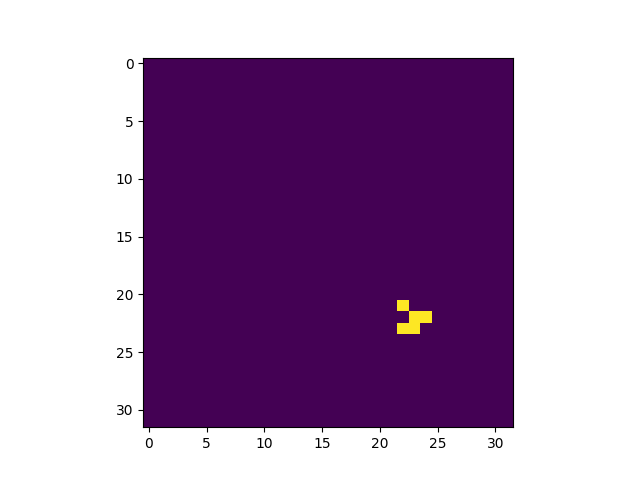
\includegraphics[width=0.7\textwidth]{glide_option.png}
\end{figure}
\clearpage
Para la \eq{2^{da}} opción resulta con el comando:
\begin{quotation}
    \centering
    {\bfseries \ttfamily python vida\_game.py --interval 500 --gosper}
\end{quotation}

El resultado es:
\begin{figure}[h]
    \centering
    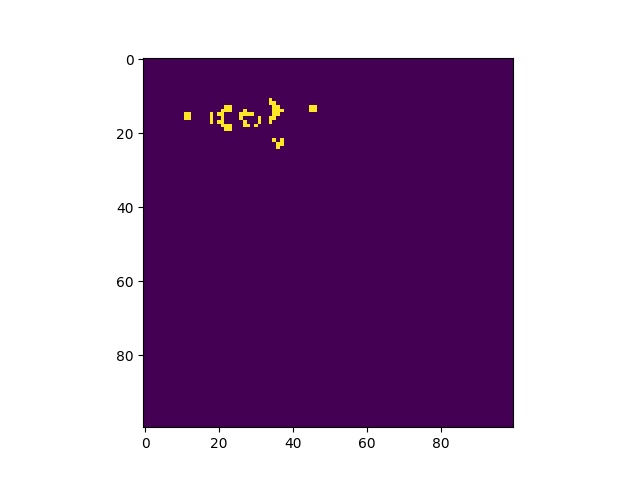
\includegraphics[width=0.7\textwidth]{gosper_option.png}
\end{figure}

Para la \eq{3^{ra}} opción resulta con el comando:
\begin{quotation}
    \centering
    {\bfseries \ttfamily python vida\_game.py --interval 500}
\end{quotation}

El resultado es:
\begin{figure}[h]
    \centering
    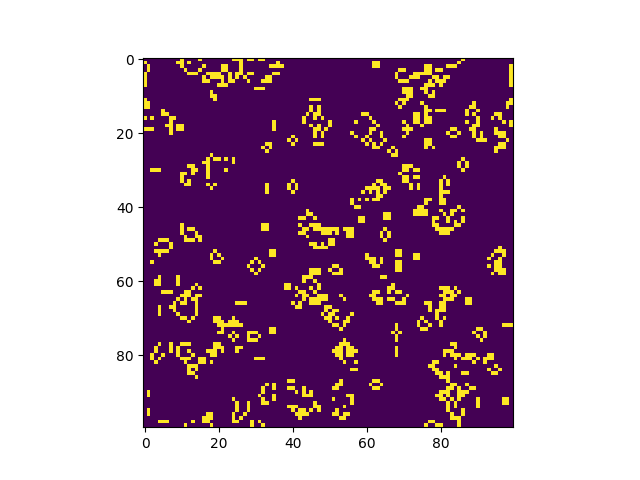
\includegraphics[width=0.6\textwidth]{random_option.png}
\end{figure}

\newpage
En la función \emph{update()}, se lleva a cabo el cambio de estado 
de cada célula siguiendo las 4 reglas de Conway explicadas anteriormente.

A continuación se muestra la implementación de esas 4 reglas y el cambio de estados.
\begin{lstlisting}
for i in range(N):
    for j in range(N):
        # calculando los vecinos
        #con fronteras periodica o toroidales.

        #el %N es para tener el comportamiento de frontera periodica
        #si es que pasa el limite las celulas en las fronteras.
        total = int((grid[i, (j-1)%N] + grid[i, (j+1)%N] +
            grid[(i-1)%N, j] + grid[(i+1)%N, j] +
            grid[(i-1)%N, (j-1)%N] + grid[(i-1)%N, (j+1)%N] +
            grid[(i+1)%N, (j-1)%N] + grid[(i+1)%N, (j+1)%N])/255)

        # aplicando las 4 reglas del juego de la vida:
        if grid[i, j] == ON:
            # < 2 vecinos muere o si es > 3 vecinos muere
            if (total < 2) or (total > 3):
                newGrid[i, j] = OFF
        else:
            #si tiene 3 vecinos revive
            if total == 3:
                newGrid[i, j] = ON
\end{lstlisting}

Y finalmente la ultima parte esta relacionada la actualización de la cuadricula del espacio
de dos dimensiones hecha a través de \emph{matplotlib}. 

En la siguiente pieza de código se especifica la función que actualizara la cuadrícula(\emph{update()}).

Se especifica, la unidad de tiempo en la que será actualizado el tablero(\emph{updateInterval}), que 
puede ser especificado por línea de comandos. 

\begin{lstlisting}
# Configuracion para el movimiento:
fig, ax = plt.subplots()
img = ax.imshow(grid, interpolation='nearest')
ani = animation.FuncAnimation(fig, update, fargs=(img, grid, N, ),
                frames = 10,
                interval=updateInterval,
                save_count=50)

# # of cuadros por segundo(fps-frames per second)
# set output file
if args.movfile:
    ani.save(args.movfile, fps=30, extra_args=['-vcodec', 'libx264'])
plt.show()
\end{lstlisting}
\newpage

\begin{thebibliography}{6}
    \bibitem{cita1} Autómatas Celulares y su Aplicación en Computación - Fernández Fraga Santiago Miguel y Rangel Mondragón Jaime. (n.d.). Retrieved July 26, 2022
    \bibitem{cita2} Autómatas Celulares. Fernando Sancho Caparrini. (n.d.). Retrieved July 26, 2022, from \url{http://www.cs.us.es/~fsancho/?e=66}.
    \bibitem{cita3} Conway's Game of Life.(Python Implementation) - GeeksforGeeks. (n.d.). Retrieved July 26, 2022, from \url{https://www.geeksforgeeks.org/conways-game-life-python-implementation/}
    \bibitem{cita4} Glider - LifeWiki. (n.d.). Retrieved July 26, 2022, from \url{https://conwaylife.com/wiki/Glider}
    \bibitem{cita5}Gosper glider gun - LifeWiki. (n.d.). Retrieved July 26, 2022, from \url{https://conwaylife.com/wiki/Gosper_glider_gun}
\end{thebibliography}
\end{document}
